\documentclass[xcolor=dvipsnames]{beamer}
\makeatletter\def\Hy@xspace@end{}\makeatother 
\usepackage{graphicx, color, amssymb, amsmath, bm, rotating, graphics,
epsfig, multicol, amsthm}
\usepackage[english]{babel}
\usepackage[T1]{fontenc}
\usepackage[ansinew]{inputenc}
\usepackage[authoryear]{natbib}
%\newcommand{\newblock}{}  %needed to make beamer and natbib play nice
\usepackage{tikz}
\usetikzlibrary{fit}  % fitting shapes to coordinates
\usetheme{Boadilla}
\usecolortheme[named=Red]{structure}
\setbeamercovered{transparent=0}
\beamertemplatenavigationsymbolsempty
\newcommand\ind{\protect\mathpalette{\protect\independenT}{\perp}}
\def\independenT#1#2{\mathrel{\rlap{$#1#2$}\mkern2mu{#1#2}}}
\newcommand\N{\mathrm{N}}
\DeclareMathOperator{\corr}{corr}
\graphicspath{{../doc/plots/}}


\title[Interweaving MCMC Strats for DLMs]{Interweaving Markov Chain Monte Carlo Strategies for Efficient
Estimation of Dynamic Linear Models}
%\subtitle{}
\author[Matt Simpson]{Matthew Simpson}
\date{January 29, 2015}
\institute[]{Departments of Statistics and Economics, Iowa State University}


%\title[short title]{long title}
%\subtitle[short subtitle]{long subtitle}
%\author[short name]{long name}
%\date[short date]{long date}
%\institution[short name]{long name}

% very important to use option [fragile] for frames containing code output!

\begin{document}


\begin{frame}
\titlepage
\begin{center}
with Jarad Niemi and Vivekananda Roy\\~\\
\scriptsize{Department of Statistics, Iowa State University}
\end{center}
\end{frame}

\begin{frame}
\frametitle{Outline}
\begin{enumerate}
\item Preliminaries\\~\\
\item Motivating example\\~\\
\item Interweaving (GIS, ASIS, CIS)\\~\\
\item Dynamic linear models\\~\\
\item Augmentations in DLMs, old and new\\~\\
\item Local level model example\\~\\
\item Conclusions
\end{enumerate}
\end{frame}

\begin{frame}
\frametitle{Preliminaries: The Basic Problem}
Bayesian statistics in a nutshell:\\~\\
\begin{enumerate}
\item Model data $y$ with a family of probability densities indexed by parameter $\phi\in\Phi$:
\begin{align*}
p(y|\phi) && \mbox{"likelihood"}
\end{align*}\\~

\pause \item Want to estimate $\phi$ -- put a probability distribution on it:
\begin{align*}
p(\phi) && \mbox{"prior"}
\end{align*}\\~

\pause \item Now apply Bayes' rule:
\begin{align*}
p(\phi|y) = \frac{p(y|\phi)p(\phi)}{\int_{\Phi}p(y|\phi)p(\phi)d\phi} && \mbox{"posterior"}
\end{align*}
\end{enumerate}
\end{frame}

\begin{frame}
\frametitle{Preliminaries: Inference and the Posterior}
Use the posterior for...

\begin{itemize}
\item Point estimates: 
\begin{align*}
\mbox{Posterior mean: } && E[\phi|y]=\int_{\Phi}\phi p(\phi|y) d\phi
\end{align*}
\pause \item Interval estimates:
\begin{align*}
\mbox{95\% credible interval: } && L,\ U\ : P(L<\phi < U) = \int_{L}^{U}p(\phi|y)d\phi
\end{align*}
\pause \item Uncertainty quantification:
\begin{align*}
\mbox{Posterior probabilities: } && P(\phi \in A|y) = \int 1(\phi\in A) p(\phi|y)d\phi
\end{align*}
\pause \item Decision theory:
\begin{align*}
\mbox{Optimal Bayes decision rule: } && d^{Bayes} = \arg\max_{d\in\mathcal{D}}E[U(d,\phi)|y]
\end{align*}
\end{itemize}

\end{frame}

\begin{frame}
\frametitle{Preliminaries: The problem}
\begin{align*}
p(\phi|y) = \frac{p(y|\phi)p(\phi)}{\int_{\Phi}p(y|\phi)p(\phi)d\phi}
\end{align*}
How do you compute the denominator?\\~\\

\pause 
\begin{itemize}
\item Numerical integration\\~\\
\pause \item Monte Carlo integration\\~\\
\pause \item Markov chain Monte Carlo integration (MCMC)
\end{itemize}
\end{frame}

\begin{frame}
\frametitle{Preliminaries: MCMC in a Nutshell}
Suppose we have some target density {\color{blue} $\pi(\phi)$} on $\Phi$ and we wish to estimate quantities of the form 
\begin{align*}
E_{\color{blue}\pi} h(\phi) = \int_{\Phi} h(\phi){\color{blue}\pi(\phi)}d\phi
\end{align*}
for some know function $h:\Phi\to\Re$.\\~\\

\pause Markov chain Monte Carlo: Simulate a Markov chain $\{\phi_n\}_{n\geq 0}$ with Markov transition density $k(\phi'|\phi)$ on $\Phi$ with invariant probability measure ${\color{blue}\pi}$.\\~\\

\[
\int_{\Phi}k(\phi'|\phi){\color{blue}\pi(\phi)}d\phi = {\color{blue}\pi(\phi')}
\]


\pause Then use the estimator
\begin{align*}
\hat{h}_k=\frac{1}{n}\sum_{i=0}^{n-1}h(\phi_i).
\end{align*}

\end{frame}

\begin{frame}
\frametitle{Preliminaries: Example Markov Chain}
Suppose $\phi=(\phi_1,\phi_2)\in\Re^2$.\\~\\

The Gibbs sampler -- obtain $(\phi_1^{(t+1)},\phi_2^{(t+1)})$ from $(\phi_1^{(t)},\phi_2^{(t)})$ by:\\~\\
\begin{enumerate}
\item Simulate:
\[
\phi_1^{(t + 1)} \sim \pi(\phi_1|\phi_2=\phi_2^{(t)})
\]
\\~\\
\item Simulate:
\[
\phi_2^{(t + 1)} \sim \pi(\phi_2|\phi_1=\phi_1^{(t+1)})
\]\\~\\
\end{enumerate}
Iterate until convergence and Monte Carlo error estimating $\hat{h}_k$ is small.
\end{frame}

\begin{frame}
\frametitle{Preliminaries: Some Markov Chain Theory}
$\{\phi_n\}_{n\geq 0}$ satisfies the usual regularity conditions (URCs) if it's irreducible, aperiodic, and Harris recurrent. \\~\\

\pause URCs $\implies$ $\hat{h}_k \stackrel{a.s.}{\to} E_{\color{blue}\pi}h(\phi)$ for all $h\in L^1({\color{blue}\pi})$.\\~\\
URCs + geometric ergodicity $\implies$ 
\[
\sqrt{n}\left(\frac{\hat{h}_k - E_{\color{blue}\pi}h(\phi)}{\sqrt{v(h,k)}}\right) \to \mbox{N}(0,1)
\]
for $h\in L^2({\color{blue}\pi})$ where $v(h,K)$ denotes the asymptotic variance of $\hat{h}_K$ under the Mtd $k(\phi'|\phi)$.\\~\\

\pause Two problems: convergence and mixing.
\begin{itemize}
\item[] Convergence: how long until $p(\phi^{(t)})$ and ${\color{blue}\pi(\phi)}$ are close?
\item[] Mixing: how much does the chain move around the space?
\end{itemize}

\end{frame}

\begin{frame}
\frametitle{Preliminaries: Data Augmentation}
Suppose it's difficult to construct a useful Markov chain with invariant density ${\color{blue}\pi(\phi)}$.\\~\\

Suppose further that there exists a density $\pi(\phi,\theta):\Phi\times\Theta\to [0,\infty)$ such that
\[
\int_{\Theta}\pi(\phi,\theta)d\theta = {\color{blue}\pi(\phi)}.
\]
\\~

\pause Data augmentation algorithm \citep{tanner1987calculation} based on $\theta$:
\[
k(\phi'|\phi)=\int_{\Theta}\pi(\phi'|\theta)\pi(\theta|\phi)d\theta
\]
with steps:
\[
[\theta|\phi]\to[\phi'|\theta]
\]
\end{frame}

\begin{frame}
\frametitle{Preliminaries: Data Augmentation -- Examples}

Often there exists natural missing data for the problem:
\begin{itemize}
\item Discrete choice models: latent unobserved continuous variable.\\
e.g. for 
\begin{align*}
y_i^*&\sim N(x_i'\beta,1); &y_i=1(y_i^*>0)
\end{align*}
the missing data is $y_{1:I}^*$.
\pause\item Hierarchical models: random effects.\\
e.g. for
\begin{align*}
y_{ij}|\alpha_j&\sim N(\alpha_j + x_{ij}'\beta, \sigma^2); &\alpha_j\sim N(\alpha_0,\tau^2)
\end{align*}
the missing data is $\alpha_{1:J}$.
\pause\item Statespace models: latent states.\\
e.g. for
\begin{align*}
y_t|\theta_t&\sim N(\theta_t,V); &\theta_t|\theta_{t-1}\sim N(\theta_{t-1},W)
\end{align*}
the missing data is $\theta_{0:T}$.
\end{itemize}
\end{frame}



\begin{frame}
\frametitle{Interweaving: A Motivating Example}
Adapted from \citet{yu2011center}, suppose:\\
\begin{align*}
y|\theta_1, \mu & \sim \N(\theta_1, 1) \\
\theta_1|\mu & \sim \N(\mu, \sigma^2) 
\end{align*}\\~\\
with $\sigma^2$ known and $p(\mu)\propto 1$.\\~\\~\\

Posterior of $\mu$: $\mu|y \sim \N(y,1+\sigma^2)$

\end{frame}

\begin{frame}
\frametitle{Interweaving: A Motivating Example}

DA algorithm based on $\theta_1$:
\begin{align*}
\theta_1|\mu,y &\sim \N\left(\frac{\mu + \sigma^2y}{1+\sigma^2}, \frac{\sigma^2}{1+\sigma^2}\right)\\
\mu |\theta_1, y &\sim \N(\theta_1, \sigma^2)
\end{align*}\\~\\

\pause Let $\theta_2 = \theta_1 - \mu$. Then DA algorithm based on $\theta_2$:
\begin{align*}
\theta_2|\mu,y &\sim \N\left(\frac{\sigma^2(\mu - y)}{1+\sigma^2}, \frac{\sigma^2}{1+\sigma^2}\right)\\
\mu |\theta_2, y &\sim \N(y-\theta_2, 1)
\end{align*}
\end{frame}

\begin{frame}
\frametitle{Interweaving: A Motivating Example}
$\sigma^2=\frac{1}{1000}$
\begin{center}
\includegraphics[width=0.9\textwidth]{trace1}\\
\end{center}
$\sigma^2=1000$
\begin{center}
\includegraphics[width=0.9\textwidth]{trace2}
\end{center}
\end{frame}

\begin{frame}
\frametitle{Interweaving: A Motivating Example}
Alternate between two DAs (alternating algorithm):
\begin{align*}
{\color{blue}[\theta_1|\mu,y]} \to {\color{blue}[\mu|\theta_1,y]} \to [\theta_2|\mu,y]\phantom{\theta_1} \to [\mu|\theta_2,y]
\end{align*}\\~\\
\pause Weave two DAs together (interweaving algorithm):
\begin{align*}
{\color{blue}[\theta_1|\mu,y]} \to {\color{blue}[\mu|\theta_1,y]} \to {\color{red}[\theta_2|\mu,\theta_1,y]} \to [\mu|\theta_2,y]
\end{align*}\\~\\\pause
The interweaving algorithm obtains {\bf IID} draws from the posterior of $\mu$.
\end{frame}


\begin{frame}
\frametitle{Global Interweaving Strategy (GIS)}

The Global Interweaving Strategy (GIS) has the Mtd
\begin{align*}
k_G(\phi'|\phi) = \int_{\Theta_2}\int_{\Theta_1}\pi(\phi'|\theta_2)\pi(\theta_2|\theta_1)\pi(\theta_1|\phi)d\theta_1d\theta_2
\end{align*}
with the steps
\begin{align*}
[\theta_1|\phi] \to \hspace{1cm} [\theta_2|\theta_1] \hspace{1.3cm} \to [\phi|\theta_2]
\end{align*}\\~\\
\pause or for ease of implementation:\\~
\begin{align*}
[\theta_1|\phi] \to [\phi|\theta_1] \to {\color{blue}[\theta_2|\theta_1,\phi]} \to [\phi|\theta_2]
\end{align*}
\end{frame}

\begin{frame}
\frametitle{Properties of GIS}
\begin{theorem}[\citet{yu2011center}]
Suppose that we have two DA schemes $\theta_1$ and $\theta_2$ such that the probability distribution $P(\phi,\theta_1,\theta_2)$ is well defined. Then
\begin{align*}
r_{G}\leq \mathcal{R}(\theta_1,\theta_2)\sqrt{r_1r_2}
\end{align*}
where
\begin{align*}
\mathcal{R}(\theta_1,\theta_2) = \sup_{h\in L_0^2(f_{\theta_1}),\ g\in L_0^2(f_{\theta_2})} \corr(h(\theta_1),g(\theta_2)).
\end{align*}
\end{theorem}
\pause
\begin{enumerate}
\item GIS converges at least as fast as the slowest of the two underlying DA algorithms.\\~
\item Control $\mathcal{R}$ $\implies$ improve convergence rate.
\end{enumerate}
\end{frame}

\begin{frame}
\frametitle{GIS and the Sandwich Kernel}

When $\Theta_1=\Theta_2$ and $\pi(\phi|\theta)=\pi(\phi|\theta)$ the GIS kernel is a sandwich kernel \citep{hobert2008theoretical,hobert2011comment}.\\~\\
\begin{itemize}
\item[] The middle step is a single move of a Markov chain on $\Theta$
\end{itemize}

\begin{theorem}[\citet{hobert2008theoretical}]
Suppose $R$ and $S$ are Mtd's on $\Theta$ with $\pi(\theta)=\int_\Phi \pi(\phi,\theta)d\phi$ as an invariant density. Let $k_R$ denote the Mtd of the sandwhich kernel based on $R$ and similarly for $S$ and assume that for all $h\in L^2_0(f_\Theta)$
\begin{align*}
\corr_{k_R}(h(\phi'),h(\phi)) < \corr_{k_S}(h(\phi'),h(\phi))
\end{align*}
Then under URCs on the $k_R$ and $k_S$ if both are reversible wrt ${\color{blue}\pi(\phi)}$ 
\begin{enumerate}
\item $v(h,k_R)\leq v(h,k_S)$ for all $h\in L^2({\color{blue}\pi(x)})$.
\item In addition if $k_R$ and $k_S$ are both DA algorithms, then $r_R\leq r_S$.
\end{enumerate}
\end{theorem}

\end{frame}


\begin{frame}
\frametitle{Ancillary-Sufficiency Interweaving Strategy (ASIS)} 

Control $\mathcal{R}(\theta_1,\theta_2)$ in GIS by requiring that one DA is a sufficient augmentation (SA) and the other is an ancillary augmentation (AA).\\~\\

Suppose we have data $y$ with the probability model $p(y,\theta|\phi)$. Then:\\~
\begin{itemize}
\item$\theta$ is an SA if $p(y|\theta,\phi)=p(y|\theta)$ (AKA centered augmentation)\\~\\
\item$\theta$ is an AA if $p(\theta|\phi)=p(\theta)$ (AKA non-centered augmentation)\\~\\
\end{itemize}
\pause Basu's theorem suggests the form and amount of dependence between an SA and an AA will be limited.
\end{frame}

\begin{frame}
\frametitle{ASIS is Optimal PX-DA}
Parameter expanded data augmentation (PX-DA): Let $M_\alpha(\theta;\phi):\Theta\to\Theta$ denote a class of transformations indexed by $\alpha$.\\~\\

Can choose the $\alpha$ that yields to the best DA algorithm \citep{meng1999seeking}...\pause or put a ``working prior'' on $\alpha$ and choose the prior that yields the best algorithm \citep{meng1999seeking,liu1999parameter}\\~\\


\begin{theorem}[\citet{yu2011center}]
Suppose $\theta_1$ is an SA and $\theta_2$ is an AA linked by a one-to-one and continuously differentiable transformation $\theta_2=M(\theta_1;\phi)$. Further assume that:
\begin{enumerate}
\item $\Phi$ forms a group, induced by $M(;\phi)$, with a unimodular Haar measure;
\item The prior density $p_0(\phi)$ wrt the Haar measure satisfies $p_0(\phi\cdot\phi')\propto p_0(\phi)p_0(\phi')$.
\end{enumerate}
Then ASIS is identical to the optimal PX-DA algorithm.
\end{theorem}
\end{frame}

\begin{frame}
\frametitle{Componentwise Interweaving Strategy (CIS)}
Finding an SA--AA pair for $\phi$ is often difficult.\\~\\

Solution: break $\phi=(\phi_1,\phi_2)$ into sub-blocks, then apply GIS or ideally ASIS separately to each block.\\~\\

For example if $\theta_1$, $\theta_2$, $\gamma_1$, and $\gamma_2$ are DAs:\\

\begin{align*}
&[\theta_1|\phi_1,\phi_2]\phantom{\theta_2,}\hspace{.06cm} \to [\phi_1|\phi_2,\theta_1\hspace{.05cm}] \to {\color{blue}[\theta_2|\phi_1,\phi_2,\theta_1]} \to [\phi_1|\phi_2,\theta_2]\to\\
&\\
&{\color{blue}[\gamma_1|\phi_1,\phi_2,\theta_2]} \to [\phi_2|\phi_1,\gamma_1] \to {\color{blue}[\gamma_2|\phi_1,\phi_2,\gamma_1]} \to [\phi_2|\phi_1,\gamma_2]\\
\end{align*}

\end{frame}

\begin{frame}[fragile]
  \frametitle{The Dynamic Linear Model} 
  For $t=1,2,...,T$
  \begin{align*}
    y_t  =&F_t\theta_t +  v_t  \qquad \mbox{(observation equation)}\\
    \theta_t =& G_t\theta_{t-1} + w_t \qquad \mbox{(system equation)}
  \end{align*} 
  with $v_t\stackrel{iid}{\sim}\N_k(0,V)$ independent of $w_t\stackrel{iid}{\sim}\N_p(0,W)$.\\~\\

\begin{figure}
  \centering
    \tikzstyle{state}=[circle, thick, minimum size=1.2cm, draw=black!80]
    \tikzstyle{obs}=[circle, thick, minimum size=1.2cm, draw=black!80]
  \begin{tikzpicture}[>=latex,text height=1.5ex,text depth=0.25ex]
    \matrix[row sep=0.5cm,column sep=0.5cm]{
    % First line: Observations
    &
    \node (y_t-1) [obs]{$y_{t-1}$}; &
    &
    \node (y_t) [obs]{$y_{t}$}; &
    &
    \node (y_t+1) [obs]{$y_{t+1}$}; &
    \\
    % Second line: States
    \node (theta_t-2) {$\cdots$}; &
    \node (theta_t-1) [state]{$\theta_{t-1}$}; &
    &
    \node (theta_t) [state]{$\theta_{t}$}; &
    &
    \node (theta_t+1) [state]{$\theta_{t+1}$}; &
    \node (theta_t+2) {$\cdots$}; \\
    };
    
    % The diagram elements are now connected through arrows:
    \path[->]
    (theta_t-2) edge (theta_t-1)
    (theta_t-1) edge (theta_t)
    (theta_t) edge (theta_t+1)
    (theta_t+1) edge (theta_t+2)
    (theta_t-1) edge (y_t-1)
    (theta_t) edge (y_t)
    (theta_t+1) edge (y_t+1)
    ;
  \end{tikzpicture}
  \end{figure}

For convenience define $y\equiv(y_1',\cdots,y_T')'$ and $\theta\equiv(\theta_0',\cdots,\theta_T)'$.

\end{frame}

\begin{frame}
  \frametitle{The Dynamic Linear Model} 
Let $\phi=(V,W)$ denote the unknown parameter.\\~\\

Priors: independently \\~\\
\begin{itemize}
\item[]$\theta_0\sim \N_p(m_0,C_0)$, $V\sim \mathrm{IW}(\Lambda_V,\lambda_V)$, and $W\sim \mathrm{IW}(\Lambda_W,\lambda_W)$\\~\\
\end{itemize}

\pause Want to apply GIS and ASIS in particular\pause, but...
\begin{theorem}
Suppose $\eta$ is a SA and $p(y,\eta|\phi)$ is Gaussian with covariance matrix
\begin{align*}
\Omega = \begin{bmatrix}   \Omega_\eta & \Omega_{y,\eta}' \\
   \Omega_{y,\eta} & \Omega_y \end{bmatrix}
\end{align*}
and let $A=\Omega_{y,\eta}'\Omega_{\eta}^{-1}$. Then if $A'A$ is invertible, $p(\phi|\eta,y)$ and $p(\phi|y)$ have a similar form.
\end{theorem}

\end{frame}

\begin{frame}
\frametitle{Data Augmentations for the DLM}
Standard DA: states $\theta$. In terms of $\theta$, the model is:
\begin{align*}
y_t|\theta,V,W \stackrel{ind}{\sim} & \N_k(F_t\theta_t,V)\\ 
\theta_t|\theta_{0:(t-1)},V,W \sim & \N_p(G_t\theta_{t-1},W)
\end{align*} 
{\color{blue}$\theta$ is an SA for $W|V$ and an AA for $V|W$.}\\~\\

\pause Scaled disturbances $\gamma\equiv(\gamma_0',\cdots,\gamma_T)'$ \citep{fruhwirth2004efficient}.
\begin{itemize}
\item[]$\gamma_0=\theta_0$ and $\gamma_t=L_W^{-1}(\theta_t - G_t\theta_{t-1})=L_W^{-1}w_t$ where $L_W$ is the Cholesky decomposition of $W$.
\end{itemize}
Then:
\begin{align*}
y_t|\gamma,V,W \stackrel{ind}{\sim} & \N_k(F_t\theta_t(\gamma,W),V) \\
\gamma_t|V,W \stackrel{iid}{\sim} & \N_p(0,I_p)
\end{align*} 

{\color{blue}$\gamma$ is an AA for $(V,W)$.}

\end{frame}

\begin{frame}
\frametitle{New Data Augmentations for the DLM}
Scaled errors $\psi\equiv(\psi_0',\cdots,\psi_T')'$:\\~\\
\begin{itemize}
\item[]$\psi_0=\theta_0$ and $\psi_t=L_V^{-1}(y_t - F_t\theta_t)=L_V^{-1}v_t$ where $L_V$ is the Cholesky decomposition of $V$.\\~\\
\end{itemize}
 
In terms of $\psi$ the model is:
\begin{align*}
y_t|\psi,V,W \stackrel{ind}{\sim} &\N_p(\mu_t(\psi,V),F_tWF_t')\\
\psi_t|V,W \stackrel{iid}{\sim} &\N_p(0,I_p)
\end{align*} 
where $\mu_t(\psi,V)$ is complicated.\\~\\

{\color{blue}$\psi$ is an AA for $(V,W)$.}
\end{frame}

\begin{frame}
\frametitle{New Data Augmentations for the DLM}
Wrongly-scaled disturbances $\tilde{\gamma}\equiv(\tilde{\gamma}_0',\cdots,\tilde{\gamma}_T')'$:\\~\\
\begin{itemize}
\item[]$\tilde{\gamma}_0=\theta_0$ and $\tilde{\gamma}_t=L_V^{-1}(\theta_t - G_t\theta_{t-1})=L_V^{-1}w_t$\\~\\
\end{itemize}

Wrongly-scaled errors $\tilde{\psi}\equiv(\tilde{\psi}_0',\cdots,\tilde{\psi}_T')'$:\\~\\
\begin{itemize}
\item[]$\tilde{\psi}_0=\theta_0$ and $\tilde{\psi}_t=L_W^{-1}(y_t - F_t\theta_{t})=L_W^{-1}v_t$\\~\\
\end{itemize}

{\color{blue} $\tilde{\gamma}$ is an SA for $W|V$ and $\tilde{\psi}$ is an SA for $V|W$.}
\end{frame}

\begin{frame}
\frametitle{Available Algorithms for DLMs}
\begin{itemize}
\item DA algorithms based on any one of the available DAs. (States, SDs, SEs, WSDs, and WSEs).
\begin{itemize}
\item Separate Gibbs steps for $V$ and $W$ often required.
\end{itemize}
\end{itemize}
\pause\begin{itemize}
\item Alternating algorithms based on any 2+ of the available DAs.
\end{itemize}
\begin{itemize}
\item GIS algorithms based on any 2+ of the available DAs.
\end{itemize}
\pause\begin{itemize}
\item One CIS algorithm using the SDs \& W-SDs for $W$ and the SEs \& W-SEs for $V$.
\end{itemize}
\pause
\begin{itemize}
\item Two partial CIS algorithms -- interweave for one of $V$ and $W$ and a normal Gibbs step for the other.\\~
\end{itemize}

\pause CIS and SD-SE GIS are equivalent up to a reordering of steps.

\end{frame}

\begin{frame}[fragile]
\frametitle{Evaluating the Strategies: the Local Level Model}
Model: for $t=1,2,...,T$
\begin{align*}
    y_t|\theta  \stackrel{ind}{\sim}&\N(\theta_t,V) \qquad (\mbox{observation equation})\\
    \theta_t|\theta_{0:(t-1)} \sim& \N(\theta_{t-1},W) \qquad (\mbox{system equation})
  \end{align*} 

Let $V^*$ and $W^*$ denote the true values used to simulate the time series.\\~\\

Independent priors:
\begin{itemize}
\item $\theta_0\sim N(0, 10^7)$, $V\sim IG(5, 4V^*)$ and $W\sim IG(5, 4W^*)$.\\~\\
\end{itemize}

Simulation Setup:
\begin{itemize}
\item Simulated data: $T=10$, $T=100$ \& $T=1000$ and $V^*$, $W^*$ $=10^{i/2}$ with $i=-4,-3,\cdots,4$.
\item Each sampler was used to fit the model to each dataset using one Markov chain started at $(V^*,W^*)$.
\end{itemize}


\end{frame}

\begin{frame}
\frametitle{LLM Results --- ESP $=$ ESS$/n$ for $T=100$}
\centering
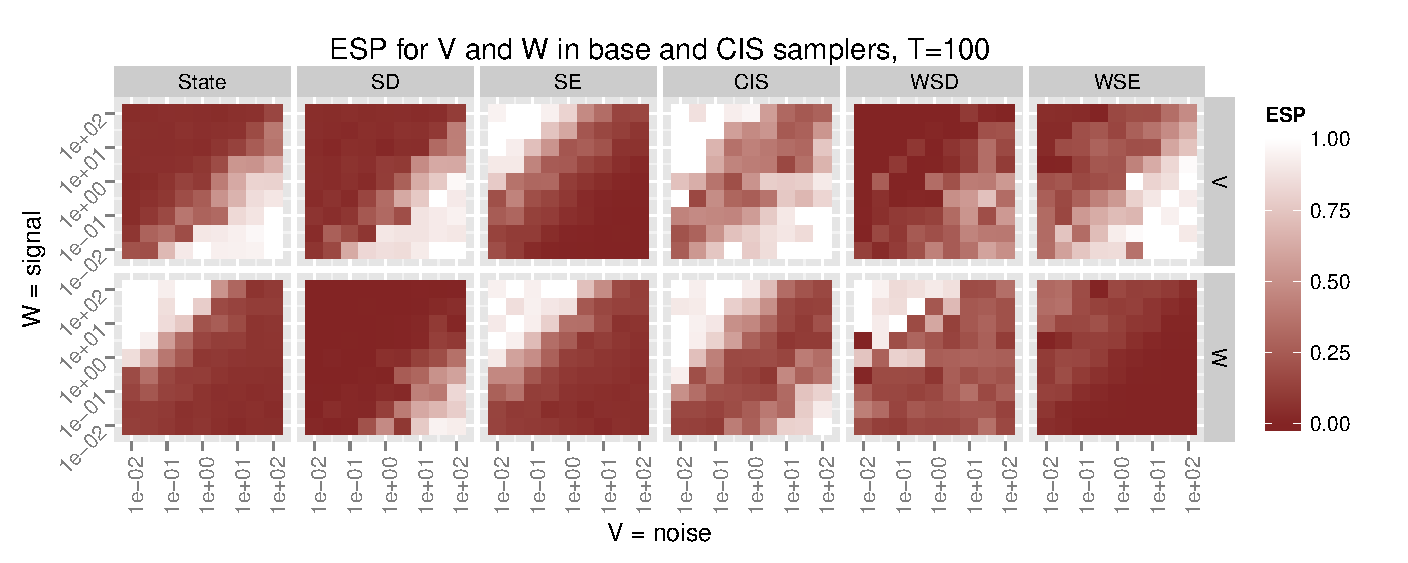
\includegraphics[width=0.59\textwidth]{../../doc/plots/basecisESplot100}\\
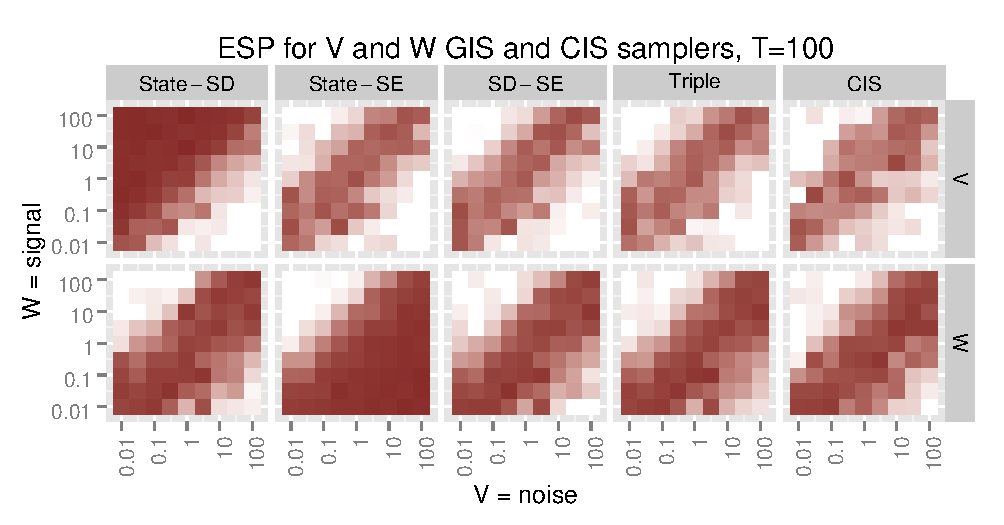
\includegraphics[width=0.53\textwidth]{../../doc/plots/altintESplotV100}
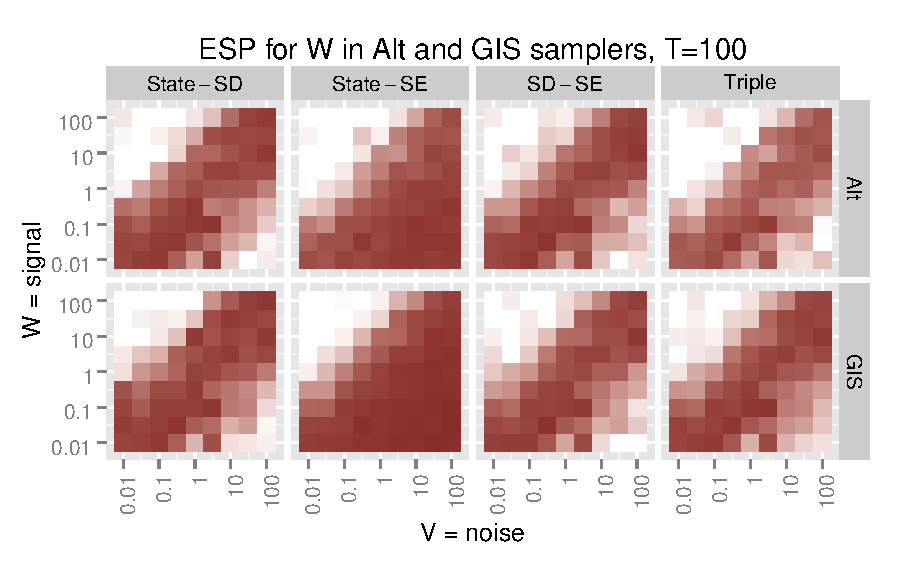
\includegraphics[width=0.45\textwidth]{../../doc/plots/altintESplotW100}
\end{frame}

\begin{frame}
\frametitle{Conclusions}
\begin{itemize}
\item Fully implementing ASIS is difficult in DLMs.\\~\\
\begin{itemize}
\item[]Also probably in hierarchical and other models with unknown variances on multiple levels.\\~\\
\end{itemize}

\item Novel DAs for DLMs: scaled errors, wrongly-scaled disturbances, and wrongly-scaled errors.\\~\\

\item GIS and Alternating also have similar {\it mixing} properties...\\~\\

\item ...but GIS is computationally cheaper than Alternating.\\~\\

\item The mixing properties of CIS are similar to SD-SE GIS.

\end{itemize}
\end{frame}

\appendix
\newcounter{finalframe}
\setcounter{finalframe}{\value{framenumber}}

\begin{frame}

      \begin{center}

        \font\endfont = cmss10 at 25.40mm
        \color{Red}
        \endfont 
        \baselineskip 20.0mm

        Thank you!

      \end{center}    


\end{frame}

\begin{frame}
\frametitle{Moving Forward: Computational Issues}
Major bottleneck: drawing from $p(W|V,\gamma,y)$ and $p(V|W,\psi,y)$:
\begin{align*}
p(x)\propto {\color{blue}x^{-\alpha-1}}\exp[-ax + b\sqrt{x} {\color{blue}- c/x}] 
\end{align*}
What about when $V$ and $W$ are matrices?\\~

$\to$ Need a better prior. E.g. $\pm \sqrt{V} \sim \N(0,\Lambda_V)$\\~\\

Then in the LLM $p(V|W,\theta,y)=p(V|W,\gamma,y)$ is GIG:
\begin{align*}
p(y) \propto y^{\alpha-1}\exp\left[-\frac{1}{2}(ay + b/y)\right] \qquad \alpha\in\Re; a,b,y>0
\end{align*}
What about when $V$ is a matrix?
\end{frame}

\begin{frame}
\frametitle{Moving Forward: Augmenting $F_t$}
Suppose $F_t=\begin{bmatrix}1 & x_t\end{bmatrix}$ and $G_t=1$:
\begin{align*}
y_t &= \begin{bmatrix}1 & x_t\end{bmatrix}\begin{bmatrix}\alpha_t \\ \beta_t\end{bmatrix} + v_t, \qquad v_t\stackrel{iid}{\sim}\N_1(0,V)\\
\begin{bmatrix}\alpha_t \\ \beta_t\end{bmatrix} &= \begin{bmatrix}\alpha_{t-1} \\ \beta_{t-1}\end{bmatrix} + \begin{bmatrix}w_{1,t} \\ w_{2,t}\end{bmatrix}, \qquad \begin{bmatrix}w_{1,t} \\ w_{2,t}\end{bmatrix}\sim\N_2(0,W)
\end{align*}
Easy way to augment the model:
\begin{align*}
\begin{bmatrix}y_t \\ y_t^*\end{bmatrix} &= \begin{bmatrix}1 & x_t\\ 0 & 1\end{bmatrix}\begin{bmatrix}\alpha_t \\ \beta_t\end{bmatrix} + \begin{bmatrix}v_t \\ v_t^* \end{bmatrix}, \qquad \begin{bmatrix} v_t\\ v_t^* \end{bmatrix}\stackrel{iid}{\sim}\N_2\left(0,\begin{bmatrix}V & 0 \\ 0 & 1\end{bmatrix}\right)\\
\begin{bmatrix}\alpha_t \\ \beta_t\end{bmatrix} &= \begin{bmatrix}\alpha_{t-1} \\ \beta_{t-1}\end{bmatrix} + \begin{bmatrix}w_{1,t} \\ w_{2,t}\end{bmatrix}, \qquad \begin{bmatrix}w_{1,t} \\ w_{2,t}\end{bmatrix}\sim\N_2(0,W)
\end{align*}
and add a step to draw $y_{1:T}^*|V,W,\alpha_{1:T},\beta_{1:T},y_{1:T}$.\\~\\

But is this the best way? Or even a good way?
\end{frame}

\begin{frame}[allowframebreaks]
        \frametitle{References}
        \bibliographystyle{plainnat}
        \bibliography{../../doc/dlmasis}
\end{frame} 
\setcounter{framenumber}{\value{finalframe}}
\end{document}
